\subsection{Measurement error}
In classical linear models, the predictors are often considered to be fixed
variables, or, if random, to be measured without error, either of which guarrantee
unbiasedness and consistency of the standard OLS estimators.
In practice, of course, exogenous predictor variables are often also observed
indicators, subject to error, a fact which is recognized in errors-in-variables
regression models and in more general structural equation models
but often ignored otherwise.  Ellipsoids in data space and $\beta$ space
are again well-suited to showing these effects.

\begin{figure}[htb]
 \begin{minipage}[b]{.49\linewidth}
  \centering
  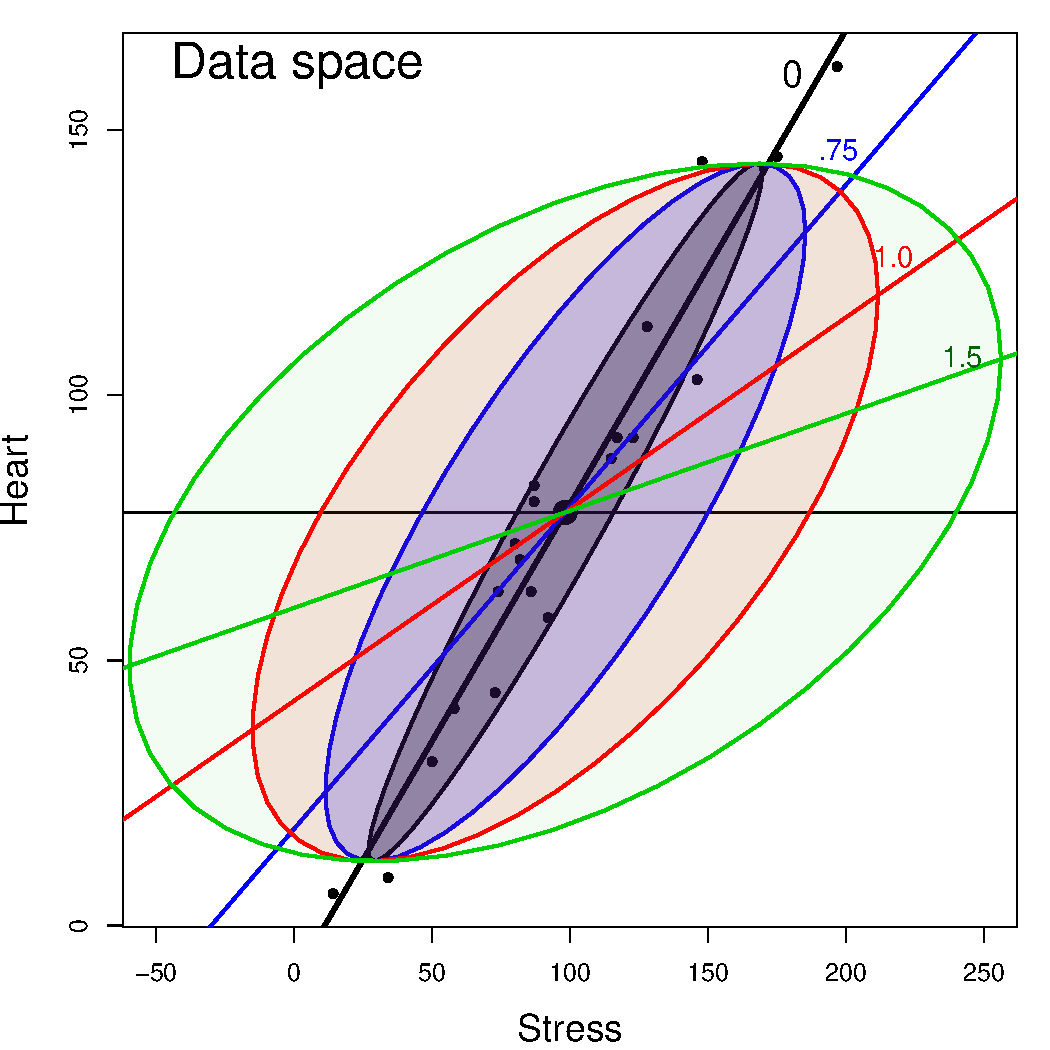
\includegraphics[width=1\linewidth]{fig/coffee-stress1}
%  \caption{}%
%  \label{fig:}
 \end{minipage}%
 \hfill
 \begin{minipage}[b]{.49\linewidth}
  \centering
  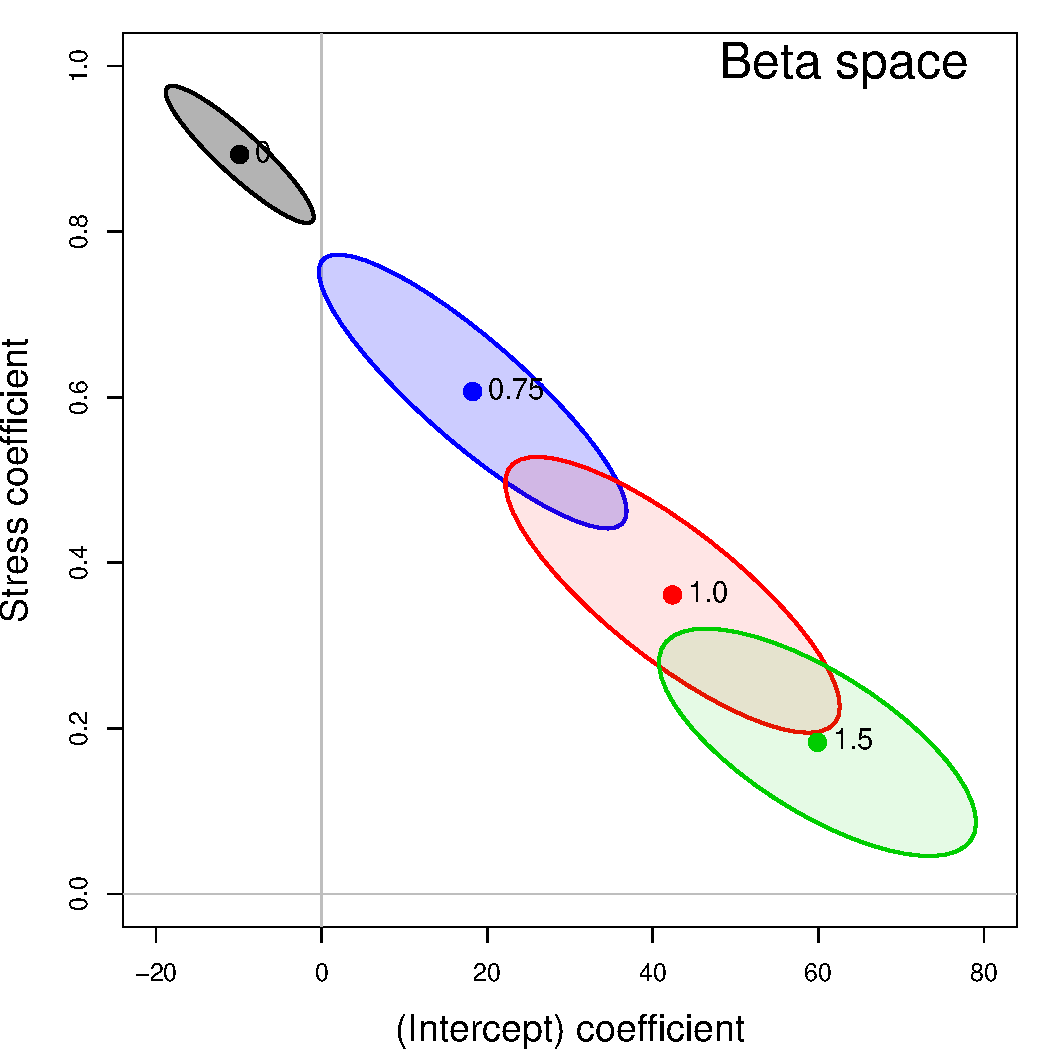
\includegraphics[width=1\linewidth]{fig/coffee-stress2}
 \end{minipage}
  \caption{Effects of measurement error in Stress on the marginal relation between Heart disease and Stress.
  Each panel starts with the observed data ($\delta=0$), then adds random normal error, 
  $\mathcal{N}(0, \delta \times SD_{Stress})$, with $\delta = \{0.75, 1.0, 1.5\}$ to the value of Stress.
  Increasing measurement error biases the slope for Stress toward 0.
  Left: 50\% data ellipses; right: 50\% confidence ellipses for $(\beta_0, \beta_{Stress})$. }
  \label{fig:coffee-stress}
\end{figure}

The statistical facts are well-known, though perhaps counter-intuitive:
measurement error in a predictor biases regression coefficients, while
increased error in the measurement of endogenous outcome $y$
variables increases the standard errors of the regression coefficients, but does not introduce
bias. 
In the top row of
\figref{fig:vis-reg-coffee11}, adding measurement error to the Heart disease variable
would expand the data ellipses vertically, but leave the slopes of the regression lines unchanged.
Measurement error in a predictor variable, however, biases the estimated coefficients toward
zero (sometimes called \emph{regression attenuation}) as well as increasing standard errors.

\figref{fig:coffee-stress} demonstrates this effect for the marginal
relation between Heart disease and stress,
with data ellipses in data space and the corresponding confidence ellipses in $\beta$ space.
Each panel starts with the observed data (the darkest ellipse, marked $0$), then adds random normal error, 
$\mathcal{N}(0, \delta \times SD_{Stress})$, with $\delta = \{0.75, 1.0, 1.5\}$ to the value of Stess,
while keeping the mean of Stress the same.
All of the data ellipses have the same vertical shadows ($s_{Heart}$), while the horizontal shadows
increase with $\delta$, driving the slope for Stress toward 0.
In $\beta$ space, it can be seen that the estimated coefficients, $(\beta_0, \beta_{Stress})$
vary along a line and would reach $\beta_{Stress}=0$ for $\delta$ sufficiently large.
The vertical shadows of
ellipses for $(\beta_0, \beta_{Stress})$ along the $\beta_{Stress}$ axis
also demonstrate the effects of measurement error
on the standard error of $\beta_{Stress}$.


